\documentclass[../../main.tex]{subfiles}
\graphicspath{{\subfix{../../image/}}} % 指定图片目录,后续可以直接使用图片文件名。

% 例如:
% \begin{figure}[H]
% \centering
% \includegraphics[scale=0.3]{image-01.01}
% \caption{图片标题}
% \label{figure:image-01.01}
% \end{figure}
% 注意:上述\label{}一定要放在\caption{}之后,否则引用图片序号会只会显示??.

\begin{document}

\section{正规子群}

\begin{definition}[正规子群]
令 $(G,\cdot)$ 是一个群,且 $N\subset G$。我们称 $N$ 是个\textbf{正规子群},记作 $N\lhd G$,若
\begin{gather*}
N\text{ 是个子群},\\
\forall a\in G, aN = Na.
\end{gather*}
\end{definition}
\begin{remark}
注意$aN=Na\nLeftrightarrow an=na,\forall n\in N.$虽然$an=na,\forall n\in N\Rightarrow aN=Na$,但是$aN=Na\nRightarrow an=na,\forall n\in N.$实际上,$aN=Na\Leftrightarrow \exists n,n' \in N\,\mathrm{s}.\mathrm{t}.\,an=n'a.$
\end{remark}

\begin{lemma}\label{lemma:子群或子幺半群与自身的乘积还等于其本身}
设 $H$ 是一个幺半群,则 $HH = H$。
\end{lemma}
\begin{note}
因为群也是幺半群,所以这个引理对群也成立。
\end{note}
\begin{proof}
一方面,对 $\forall h_1,h_2\in H$,根据乘法封闭性(乘法是$H$上的代数运算),都有 $h_1h_2\in H$。故 $HH\subset H$。

另一方面,设 $h\in H$,则 $h = he\in HH$,其中$e$是$H$的单位元.故 $H\subset HH$。
因此 $HH = H$。 
\end{proof}

\begin{proposition}\label{proposition:陪集乘法的良定义性}
令 $(G,\cdot)$ 是一个群,且 $N\lhd G$,$a,b\in G$,则
\begin{align*}
(aN)\cdot(bN)=(ab)N.
\end{align*}
是良定义的.
\end{proposition}
\begin{remark}
因为陪集代表元的不唯一性可能导致上述乘积运算结果不唯一,所以上述乘积运算不一定是良定义的,需要给出证明.
\end{remark}
\begin{conclusion}
元素与群(其实只要满足结合律的半群就足够了)的乘积满足广义结合律. 例如:
设$G$是一个群,若$H,K<G$,$a,b\in G$,则
\begin{gather*}
aHbK=(aH)(bK)=a((Hb)K)=a(H(bK))=(a(Hb))K=((aH)b)K.
\\
abHK=(ab)(HK)=a((bH)K)=a(b(HK))=((ab)H)K.
\\
\cdots \cdots \cdots \cdots
\end{gather*}
即两个陪集相乘可以看作一个陪集或两个陪集的乘积的陪集等.
\end{conclusion}
\begin{proof}
{\color{blue}证法一:}
设 $aN = a'N, bN = b'N$,则由\hyperref[lemma:关于两个陪集相等的充要条件]{引理\ref{lemma:关于两个陪集相等的充要条件}}可知$a^{-1}a',b^{-1}b'\in N$,我们只须证明 $abN = a'b'N$,即 $(ab)^{-1}a'b' = b^{-1}a^{-1}a'b'\in N$。首先中间这个部分,即 $a^{-1}a'$,是在 $N$ 中的。接着,利用 $N$ 是个正规子群,再结合\hyperref[lemma:两个相等的陪集同时左乘相同元素保持等号]{引理\ref{lemma:两个相等的陪集同时左乘相同元素保持等号}},我们可以得到 $b^{-1}Nb = N$,因此,$b^{-1}a^{-1}a'b'\in b^{-1}Nb' = N$。进一步地,由\hyperref[lemma:关于两个陪集相等的充要条件]{引理\ref{lemma:关于两个陪集相等的充要条件}}可得$abN = a'b'N$。这就证明了良定义性。

{\color{blue}证法二:}事实上,这个乘法可以简单地理解成子集乘法,即 $(aN)(bN)=\{xy:x\in aN, y\in bN\}$。我们只须说明,这从集合意义上,等于 $abN$。而这几乎是显然的。由于 $Nb = bN$及\hyperref[lemma:子群或子幺半群与自身的乘积还等于其本身]{引理\ref{lemma:子群或子幺半群与自身的乘积还等于其本身}},我们有 $aNbN = abNN = abN$.这样,既然从集合意义上相等,那么自然就是良定义的(因为我们不必选取单位元)。 
\end{proof}

\begin{proposition}[商群]\label{proposition:商群}
令 $(G,\cdot)$ 是一个群,且 $N\lhd G$,则 $(G/N,\cdot)$ 构成一个群,称为($G$ 在 $N$ 上的)\textbf{商群},其中的单位元是 $eN = N$,每个陪集 $aN$ 的逆元是 $a^{-1}N$。
\end{proposition}
\begin{proof}
由\hyperref[proposition:陪集乘法的良定义性]{命题\ref{proposition:陪集乘法的良定义性}}可知商群$(G/N,\cdot)$的乘法是良定义的.

封闭性:对$\forall aN,bN\in (G/N,\cdot)$,其中$a,b\in G$,根据$G$对乘法的封闭性可得$ab\in G$,从而$(aN)(bN)=abN\in (G/N,\cdot)$.

结合律:令 $a,b,c\in G$,则利用乘法的定义,$(aNbN)cN=(abN)(cN)=((ab)c)N$。利用 $G$ 对乘法的结合律,得到这是等于 $(a(bc))N$ 的。类似地,这最终等于 $aN(bNcN)$。

单位元:令 $a\in G$,则 $aNeN=(ae)N = aN$,类似地 $eNaN = aN$。

逆元:令 $a\in G$,则 $aNa^{-1}N=(aa^{-1})N = eN$,类似地 $a^{-1}NaN = eN$。

综上,若 $N\lhd G$,则 $G/N$ 在这个自然的乘法下构成群,称为一个商群。 
\end{proof}

\begin{lemma}[正规子群的等价条件]\label{lemma:正规子群的等价条件}
令 $(G,\cdot)$ 是一个群,且 $N < G$,则下列命题等价
\begin{enumerate}[(1)]
\item $N$ 是 $G$ 的正规子群,即
$\forall a\in G, aN = Na .$

\item $\forall a\in G, aNa^{-1}= N .$

\item
$\forall a\in G, aNa^{-1}\subset N .$

\item 
$\forall a\in G, \forall n\in N, ana^{-1}\in N .$
\end{enumerate}
\end{lemma}
\begin{proof}
显然(3)和(4)等价.

$(1)\Leftrightarrow (2)$:一方面,设 $N$ 是 $G$ 的正规子群.则由\hyperref[lemma:两个相等的陪集同时左乘相同元素保持等号]{引理\ref{lemma:两个相等的陪集同时左乘相同元素保持等号}}可得$\forall a\in G, aNa^{-1}= N .$

另一方面,设(2)成立.则由\hyperref[lemma:两个相等的陪集同时左乘相同元素保持等号]{引理\ref{lemma:两个相等的陪集同时左乘相同元素保持等号}}可得$\forall a\in G, aN = Na .$

$(1)\Leftrightarrow (3)$:
一方面,设 $N$ 是 $G$ 的正规子群。令 $a\in G$,则 $aN = Na$。同时右乘 $a^{-1}$ 并取一半的包含关系,我们得到了 $aNa^{-1}\subset N$。

另一方面,设(3)成立。令 $a\in G$,则由 $aNa^{-1}\subset N$ 及\hyperref[lemma:两个相等的陪集同时左乘相同元素保持等号]{引理\ref{lemma:两个相等的陪集同时左乘相同元素保持等号}}得到 $aN\subset Na$,由 $a^{-1}N (a^{-1})^{-1}\subset N$及\hyperref[lemma:两个相等的陪集同时左乘相同元素保持等号]{引理\ref{lemma:两个相等的陪集同时左乘相同元素保持等号}}得到得到 $Na\subset aN$。因此,$aN = Na$。 
\end{proof}

\begin{example}
证明: \(SL(n, \mathbb{R}) \lhd GL(n, \mathbb{R})\).
\end{example}
\begin{proof}
显然 \(SL(n, \mathbb{R}) < GL(n, \mathbb{R})\)。任取 \(A \in GL(n, \mathbb{R})\),\(N \in SL(n, \mathbb{R})\),都有
\begin{align*}
\det(ANA^{-1}) &= \frac{\det(A)\det(N)}{\det(A)} = \det(N) = 1.
\end{align*}
从而 \(ANA^{-1} \in SL(n, \mathbb{R})\)。故 \(SL(n, \mathbb{R}) \lhd GL(n, \mathbb{R})\)。 
\end{proof}

\begin{proposition}[正规子群的任意交还是正规子群]\label{正规子群的任意交还是正规子群}
设 $(N_i)_{i\in I}$ 是一族 $G$ 的正规子群,则它们的交集仍然是 $G$ 的正规子群,即
\begin{align*}
\bigcap_{i\in I}N_i\lhd G .
\end{align*}
\end{proposition}
\begin{proof}
首先,由\hyperref[proposition:子群的任意交仍是子群]{子群的任意交仍是子群}可知$\bigcap_{i\in I}N_i< G .$
因此我们只需证明正规性。利用\hyperref[lemma:正规子群的等价条件]{正规子群的等价条件(3)}可知,对$\forall a\in G,\forall n\in \bigcap_{i\in I}N_i$,我们只须证明$ana^{-1}\in \bigcap_{i\in I}N_i$即可.任取 $i\in I$,则 $n\in N_i$。由于 $N_i\lhd G$,我们有 $ana^{-1}\in N_i$。因此,由$i$的任意性可知$ana^{-1}\in \bigcap_{i\in I}N_i$。这就证明了 $\bigcap_{i\in I}N_i\lhd G$。
\end{proof}

\begin{proposition}\label{proposition:平凡群和整个群都是正规子群}
令 $(G,\cdot)$ 是一个群,则
\begin{align*}
\{e\}&\lhd G ,\\
G&\lhd G .
\end{align*}
\end{proposition}
\begin{proof}
平凡群:怎么乘都是单位元,所以对乘法封闭;包含单位元;唯一的元素的逆元还是单位元;在这个群中,$a$ 的左右陪集都是 $a\{e\}=\{e\}a = \{a\}$。因此,$\{e\}\lhd G$。

整个群:子群是显然的;在整个群 $G$ 中,每个元素的左右陪集都是全集,即 $aG = Ga = G$,这是因为 $a\in G$。因此,$G\lhd G$(\hyperref[corollary:关于两个陪集相等的充要条件推论]{推论\ref{corollary:关于两个陪集相等的充要条件推论}}).
\end{proof}

\begin{corollary}\label{corollary:G/{e}同构于G,G/G={e}}
\begin{enumerate}[(1)]
\item 若 $G$ 是一个群,$e$ 是其单位元,则 $G/\{e\}$ 同构于 $G$,即 $G/\{e\}\simeq G$。

\item 若 $G$ 是一个群,则 $G/G$ 是平凡群,即 $G/G = \{e\}$。
\end{enumerate}
\end{corollary}
\begin{proof}
\begin{enumerate}[(1)]
\item 令 
\[f:G\rightarrow G/\{e\}, a\mapsto a\{e\}=\{a\}.\]
显然 $f$ 是双射。对 $\forall a,b\in G$,我们都有
\begin{align*}
f(ab)&=\{ab\}=ab\{e\}=(a\{e\})(b\{e\})=\{a\}\{b\}=f(a)f(b).
\end{align*}
因此 $f$ 也是同态映射。于是 $f$ 是同构映射。故 $G/\{e\}\simeq G$。

\item 由\hyperref[proposition:商群]{命题\ref{proposition:商群}}及\hyperref[proposition:平凡群都是正规子群]{命题\ref{proposition:平凡群和整个群都是正规子群}}可知 $G/G$ 是一个群。注意到 $\forall a\in G$,都有 $aG = G$。因此 $G/G = G$。于是 $|G/G| = 1$。故 $G/G = \{e\}$。 
\end{enumerate}
\end{proof}

\begin{proposition}\label{proposition:阿贝尔群的子群与正规子群等价}
令 $(G,\cdot)$ 是个阿贝尔群,则子群就是正规子群,正规子群也就是子群,即
\begin{align*}
H < G\iff H\lhd G
\end{align*}
\end{proposition}
\begin{proof}
$\Leftarrow$:由于正规子群都是子群,故显然成立.

$\Rightarrow$:根据阿贝尔群满足交换律可知$aH = \{ah:h\in H\} = \{ha:h\in H\} = Ha$。
\end{proof}

\begin{theorem}[群同构第一定理]\label{theorem:群同构第一定理}
设 \(f: G \to G'\) 是一个群同态,则 \(\ker(f) \lhd G\),且 \(G\) 在 \(\ker(f)\) 上的商群同构于 \(\mathrm{im}(f)\),即
\begin{align*}
G/\ker(f) &\cong \mathrm{im}(f) .
\end{align*}
特别地,若 \(f\) 是满同态,则
\begin{align*}
G/\ker(f) &\cong G' .
\end{align*}
若 \(f\) 是单同态,则
\begin{align*}
G/\{e\} &\cong G \cong \mathrm{im}(f).
\end{align*}
若 \(G\) 是有限群,则
\begin{align*}
\frac{|G|}{|\ker(f)|} &= |\mathrm{im}(f)| ,\text{也即}|G|=|\ker(f)||\mathrm{im}(f)|.
\end{align*}
\end{theorem}
\begin{remark}
要注意,同态的像($\mathrm{im}(f)$)未必是$G'$的正规子群,往往只是普通的子群。
\end{remark}
\begin{proof}
根据\hyperref[proposition:一个群同态是单的当且仅当核是平凡的]{命题\ref{proposition:一个群同态是单的当且仅当核是平凡的}}和\hyperref[theorem:Lagrange定理]{Lagrange定理},这三条推论都是显然的,唯一要说明的是 \(G/\{e\}\) 为什么同构于 \(G\),这由\hyperref[corollary:G/{e}同构于G,G/G={e}]{推论\ref{corollary:G/{e}同构于G,G/G={e}}(1)}可直接得到.这就意味着我们只须证明原命题即可.

首先要说明每个同态的核都是定义域的正规子群。我们只须证明,若 \(a \in G\),\(n \in \ker(f)\),则 \(ana^{-1} \in \ker(f)\)。注意到
\begin{align*}
f(ana^{-1}) &= f(a)e'f(a)^{-1} = e' .
\end{align*}
因此 \(ana^{-1} \in \ker(f)\)。这就证明了 \(\ker(f) \lhd G\)。

接下来,我们要找到一个从商群 \(G/\ker(f)\) 到像集 \(\mathrm{im}(f)\) 的同构映射。我们称这个映射叫 \(\tilde{f}: G/\ker(f) \to \mathrm{im}(f)\),对于 \(a \in G\),定义为
\begin{align*}
\tilde{f}(a\ker(f)) &= f(a) .
\end{align*}
为了方便起见,在不会引起歧义的情况下,我们令 \(N = \ker(f)\),也即
\begin{align*}
\tilde{f}(aN) &= f(a) .
\end{align*}

考虑到陪集代表元的不唯一性,我们要证明良定义性。假设 \(aN = a'N\),或 \(a^{-1}a' \in N\),只须证明 \(f(a) = f(a')\),而这是因为
\begin{align*}
f(a') &= f(aa^{-1}a') = f(a)f(a^{-1}a') =f(a)f(eN)= f(a)e' = f(a) .
\end{align*}
其中$e$是$G$的单位元,$e'$是$G'$的单位元.这就证明了良定义性。

接下来,我们要证明 \(\tilde{f}\) 既是同态,也是双射(单射 + 满射)。

同态 :令 \(a, b \in G\),则 \(\tilde{f}(aN) = f(a)\),\(\tilde{f}(bN) = f(b)\),而由$N=\ker f \lhd G$及$f$是一个群同态可得
\begin{align*}
\tilde{f}((aN)(bN)) &= \tilde{f}(abN) = f(ab) = f(a)f(b) = \tilde{f}(aN)\tilde{f}(bN) .
\end{align*}
这就证明了 \(\tilde{f}\) 是一个同态。

单射 :只须证明 \(\ker(\tilde{f}) = \{N\}\)。设 \(\tilde{f}(aN) = e'\),则根据定义,\(f(a) = e'\),故 \(a \in \ker(f) = N\),所以 \(aN = N\),这就证明了 \(\tilde{f}\) 是一个单射。

满射 :令 \(a' \in \mathrm{im}(f)\),取 \(a \in G\) 使得 \(a' = f(a)\)。因此,\(\tilde{f}(aN) = f(a) = a'\),这就证明了 \(\tilde{f}\) 是一个满射。

综上所述,\(\tilde{f}\) 是一个从商群 \(G/\ker(f)\) 到像集 \(\mathrm{im}(f)\) 的同构。作为结论,
\begin{align*}
G/\ker(f) &\cong \mathrm{im}(f) .
\end{align*}
这就完成了整个命题的证明。 
\end{proof}
\begin{figure}[H]
\centering
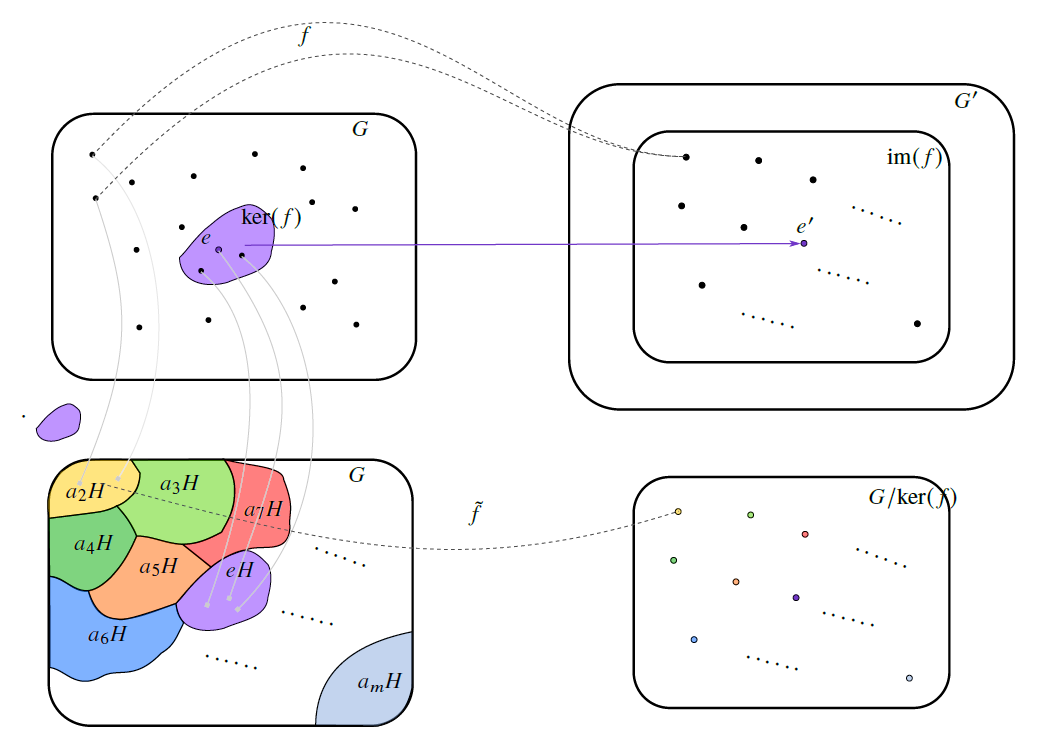
\includegraphics[scale=0.4]{群同构第一定理示意图.png}
\caption{群同构第一定理示意图}
\label{figure:群同构第一定理示意图}
\end{figure}

\begin{example}
证明:$GL(n, \mathbb{R})/SL(n, \mathbb{R})\cong \mathbb{R}^{\times}$.
\end{example}
\begin{proof}
由\hyperref[example:行列是就是一个乘法群同态]{命题\ref{example:行列是就是一个乘法群同态}}可知
\begin{align*}
\det: GL(n, \mathbb{R}) &\to \mathbb{R}^{\times}.
\end{align*}
是个满同态,且 \(\ker(\det) = SL(n, \mathbb{R})\),故由\hyperref[theorem:群同构第一定理]{群同构第一定理},我们有
\begin{align*}
SL(n, \mathbb{R}) \lhd GL(n, \mathbb{R})\text{且}GL(n, \mathbb{R})/SL(n, \mathbb{R}) &\cong \mathbb{R}^{\times}.
\end{align*} 
\end{proof}

\begin{corollary}\label{corollary:群同构第一定理推论1}
设 $G$是有限群,\(f: G \to G'\) 是一个群同态,则
\begin{align*}
\left| \mathrm{im}\,f \right|\Big | \mathrm{gcd}\left( \left| G \right|,\left| G'\right| \right) .
\end{align*}
\end{corollary}
\begin{proof}
由\hyperref[theorem:群同构第一定理]{群同构第一定理}可知,$\left| \mathrm{im}\,f \right|\Big | G$.由\hyperref[theorem:Lagrange定理]{Lagrange定理}可知,$\left| \mathrm{im}\,f \right|\Big | G'$.故
\begin{align*}
\left| \mathrm{im}\,f \right|\Big | \mathrm{gcd}\left( \left| G \right|,\left| G'\right| \right) .
\end{align*}
\end{proof}

\begin{example}
设$f:C_{12}\to C_{35}$是一个群同态,求证:$f$是平凡同态,即对$\forall x\in C_{12}$,都有$f(x)=e$,也即$\mathrm{im}\,f=\{e\}$.,其中$e$是$C_{35}$的单位元.
\end{example}
\begin{proof}
由\hyperref[corollary:群同构第一定理推论1]{推论\ref{corollary:群同构第一定理推论1}}可知,$\left| \mathrm{im}\,f \right|\Big | \mathrm{gcd}\left( 12,35 \right)=1 .$又因为$\mathrm{im}\,f<G'$,所以$\mathrm{im}\,f=\{e\}$.
\end{proof}

\begin{lemma}\label{lemma:HN<G的条件}
设 \((G, \cdot)\) 是一个群,且 \(N \lhd G\),\(H < G\)。则$HN<G$.
\end{lemma}
\begin{proof}
设 \(e\) 是 \(G\) 的单位元,则由 \(N \lhd G\),\(H < G\) 可知,\(e \in N \cap H\)。从而 \(e = ee \in HN\)。

对 \(\forall h_1n_1, h_2n_2 \in HN\),其中 \(h_1, h_2 \in H\),\(n_1, n_2 \in N\)。
由 \(N \lhd G\),\(H < G\) 可得
\begin{align*}
h_1n_1\left( h_2n_2 \right) ^{-1} &= h_1n_1n_{2}^{-1}h_{2}^{-1} = h_1n_1h_{2}^{-1}n_{2}^{-1} = h_1h_{2}^{-1}n_1n_{2}^{-1} \in HN.
\end{align*}
故 \(HN < G\).
\end{proof}

\begin{theorem}[群同构第二定理]\label{theorem:群同构第二定理}
设 \((G, \cdot)\) 是一个群,且 \(N \lhd G\),\(H < G\)。则 \(H \cap N \lhd H\),\(N \lhd HN\),且
\begin{align*}
H/(H \cap N) &\cong HN/N .
\end{align*}
这和之前两个子群乘积的阶的公式是类似的。
\end{theorem}
\begin{remark}
由\hyperref[lemma:HN<G的条件]{引理\ref{lemma:HN<G的条件}}可知$HN<G$.故此时\(N \lhd HN\)是有意义的.
\end{remark}
\begin{proof}
第一,要证明 \(H \cap N \lhd H\)。令 \(h \in H\),而 \(x \in H \cap N\),则 \(hxh^{-1} \in H\),而且因为 \(N \lhd G\),\(hxh^{-1} \in N\),因此 \(hxh^{-1} \in H \cap N\)。

第二,要证明 \(N \lhd HN\)。令 \(hn \in HN\),而 \(n' \in N\)。则由\hyperref[lemma:正规子群的等价条件]{引理\ref{lemma:正规子群的等价条件}(2)}可得\(hnn'(hn)^{-1} = h(nn'n^{-1})h^{-1} \in hNh^{-1} = N\)。

第三,要证明 \(H/(H \cap N) \cong HN/N\)。令 \(f: H \to HN/N\),定义为
\begin{align*}
f(h) &= hN .
\end{align*}
这显然是良定义的(若$h=h'\in H$,则$h^{-1}h'=e\in N$,从而$f(h)=hN=h'N=f(h')$).又由\(N \lhd G\)及\hyperref[lemma:子群或子幺半群与自身的乘积还等于其本身]{引理\ref{lemma:子群或子幺半群与自身的乘积还等于其本身}}可知,对$\forall h_1,h_2\in H$,都有
\begin{align*}
f\left( h_1h_2 \right) =h_1h_2N=h_1h_2NN=h_1Nh_2N=f\left( h_1 \right) f\left( h_2 \right) .
\end{align*}
故$f$是同态的.
根据 \(HN/N = \{hnN : h \in H, n \in N\} = \{hN : h \in H\}\)可知,$f$还是个满同态。

接下来,根据\hyperref[lemma:关于两个陪集相等的充要条件]{引理\ref{lemma:关于两个陪集相等的充要条件}}可知,$f$的核是 \(\ker(f) = \{h \in H : hN = eN\} = \{h \in H : h \in N\} = H \cap N\)。因此,根据\hyperref[theorem:群同构第一定理]{群同构第一定理},
\begin{align*}
H/(H \cap N) &\cong HN/N .
\end{align*}
这就证明了群同构第二定理。
\end{proof}

\begin{lemma}\label{lemma:正规子群的"传递性"}
设\((G, \cdot)\) 是一个群,且 \(N <G\),\(M \lhd G\),\(M < N\),则$M\lhd N.$ 
\end{lemma}
\begin{proof}
令 \(n \in N\subset G\),\(m \in M\),则由$M\lhd G$可知,\(nmn^{-1} \in M\)。因此由\hyperref[lemma:正规子群的等价条件]{引理\ref{lemma:正规子群的等价条件}}可知$M\lhd N$.
\end{proof}

\begin{theorem}[群同构第三定理]\label{theorem:群同构第三定理}
设\((G, \cdot)\) 是一个群,且 \(N \lhd G\),\(M \lhd G\),\(M < N\)。则 \(N/M \lhd G/M\),且
\begin{align*}
(G/M)/(N/M) &\cong G/N .
\end{align*}
\end{theorem}
\begin{proof}
首先显然有\(N/M \subset G/M\)。由\hyperref[lemma:正规子群的"传递性"]{引理\ref{lemma:正规子群的"传递性"}}可知$M\lhd N$.因此 \(N/M\) 是个商群。
因为这两个都是群,所以对单位元、乘法和逆元都有封闭性.因此就有 \(N/M < G/M\)。接下来我们可以先证明正规性,这也几乎是显然的。令 \(nM \in N/M (n \in N)\),\(gM \in G/M (g \in G)\),则由$M\lhd N,N\lhd G$可得
\begin{align*}
(gM)(nM)(gM)^{-1} &= (gng^{-1})M \in \{nM : n \in N\} = N/M .
\end{align*}
因此 \(N/M \lhd G/M\).

那么,我们要定义 \(f: G/M \to G/N\),定义为
\begin{align*}
f(gM) &= gN .
\end{align*}
要证明良定义性。假设 \(gM = g'M\),则 \(g^{-1}g' \in M\),故 \(g^{-1}g' \in N\),所以 \(gN = g'N\)。

同态是显然的:对$\forall gM,g'M\in G/M$,都有
\begin{align*}
f(gMg'M) &= f(gg'M) = gg'N = gNg'N = f(gM)g(g'M) .
\end{align*}
满同态几乎也是显然的。任取 \(gN \in G/N (g \in G)\),则 \(f(gM) = gN\)。

最后,注意到
\begin{align*}
\ker(f) &= \{gM : f(gM) = gN = eN\} = \{gM : g \in N\} = N/M .
\end{align*}
于是根据\hyperref[theorem:群同构第一定理]{群同构第一定理},这就告诉我们
\begin{align*}
(G/M)/(N/M) &\cong G/N.
\end{align*}
综上所述,我们就证明了群同构第三定理。 
\end{proof}











\end{document}